% Chapter Template

\chapter{Desarrollo}

\label{Chapter4} % Change X to a consecutive number; for referencing this chapter elsewhere, use \ref{ChapterX}

Una vez presentado el contexto, los objetivos, así como las herramientas empleadas y los fundamentos teóricos, en este capítulo se detalla la solución software desarrollada. Primero se presenta el diseño global y después se analiza en detalle el componente realizado con una visión profunda del desarrollo por bloques y su funcionamiento.


%-----------------------------------
%	SECTION Diseño
%-----------------------------------
\section{Diseño}

El sistema se basa principalmente en dos componentes; uno existente en JdeRobot (\textbf{OpenniServer}) que funciona como driver del sensor y proporciona las imágenes obtenidas por éste y el componente realizado en este proyecto (\textbf{RealRTEstimator}) que se encarga, una vez recogidas las imágenes, de toda la lógica restante.

El objetivo del componente, como ya se ha comentado, consiste en estimar en tiempo real la posición y movimiento incremental y el 3D del sensor, por lo que deberá entregar una estimación en todo momento.

En la Figura~\ref{fig:diagram1} se puede apreciar el diagrama global de funcionamiento del componente desarrollado y su conexión con otros componentes para los diferentes datos de entrada.

\begin{figure}[th]
\centering
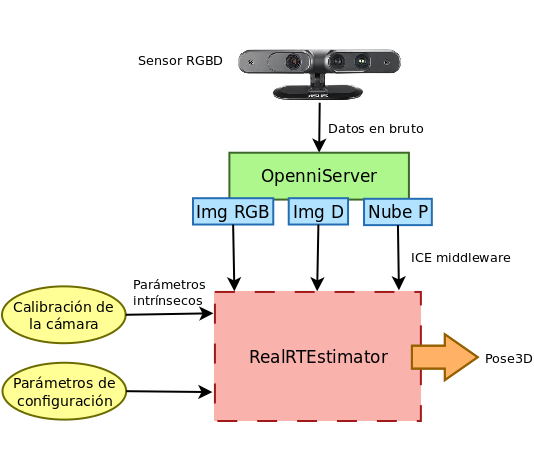
\includegraphics[scale=0.4]{Figures/diagram1.png}
\decoRule
\caption[Esquema general del componente RealRTEstimator]{Esquema global de funcionamiento, entradas y salidas.}
\label{fig:diagram1}
\end{figure}

OpenniServer se encarga de preparar y enviar las imágenes del sensor. El componente RealRTEstimator recoge las imágenes a través de ICE y es el encargado de procesarlas. También recibe los datos de los parámetros intrínsecos de la cámara así como algunos parámetros de configuración, como pueden ser la activación/desactivación de la interfaz de usuario o algunos parámetros configurables de los algoritmos internos. A su salida entrega una matriz RT que describe la posición y orientación 3D absolutas en ese preciso instante de tiempo. 

Respecto al funcionamiento interno del RealRTEstimator se puede ver a grandes rasgos el diagrama de bloques en la Figura~\ref{fig:diagram2}. Se observa el diseño implementado así como sus bloques funcionales:

\begin{figure}[!ht]
\centering
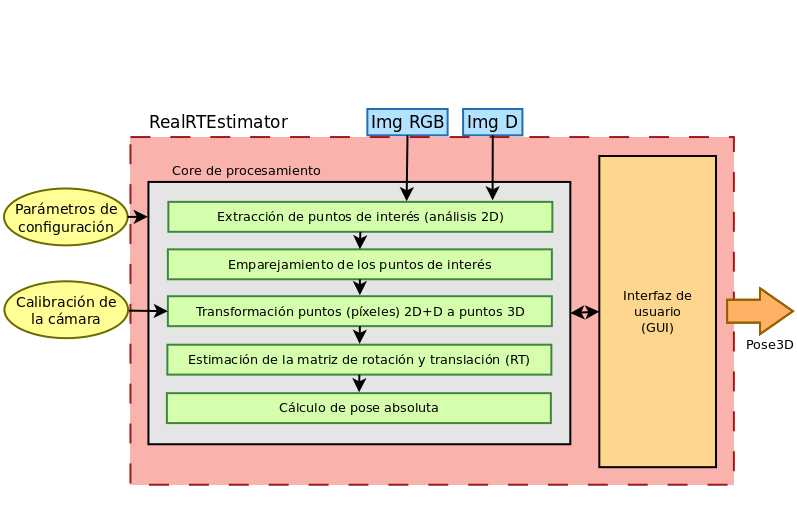
\includegraphics[scale=0.36]{Figures/diagram2.png}
\decoRule
\caption[Diagrama interno del componente RealRTEstimator]{Diagrama interno del componente RealRTEstimator.}
\label{fig:diagram2}
\end{figure}

\begin{itemize}
\item Extración de puntos de interés (análisis 2D) del fotograma actual.

\item Emparejamientos de puntos de interés en t con respecto a los puntos extraídos en el instante anterior (t-1).

\item Transformación de puntos (píxeles) en 2D usando la imagen de profundidad a nube de puntos en 3D.

\item Cálculo de movimiento. Es decir, estimación de la matriz de rotación y translación (Matriz RT).

\item Calculo de pose 3D absoluta.

\end{itemize}

En las siguientes secciones desglosaremos el funcionamiento de estos diferentes bloques funcionales.

%-----------------------------------
%	SECTION Extracción de características de una imágen
%-----------------------------------
\section{Análisis 2D}

El primer bloque del componente RealRTEstimator es el de análisis 2D. A partir de dos imágenes, imagen de color y la de profundidad, se procede a la extracción de puntos de interés.

\subsection{Detección de puntos de interés}

El término puntos de interés o detección de características (\textit{Feature Detection} en inglés) hace referencia a la tarea de localizar en una imágen puntos relevantes o carácterísticos. Estos puntos suelen ser comunes y son fáciles de seguir de fotograma en fotograma.

Para entender cuáles son estos puntos característicos podemos observar un ejemplo sencillo en la Figura~\ref{fig:feature_simple}. El cuadrado azul se encuentra en una área plana, y es difícil de seguir o encontrar. En cualquier lugar por donde se desplace parecerá que es el mismo. Para el cuadrado negro, que es un borde, igual para el desplazamiento lateral; sin embargo, para el desplazamiento vertical el punto ya cambia. Por último, está el cuadrado rojo, que es una esquina. Para cualquier desplazamiento de esta figura, el punto ya es diferente, lo que significa que ese punto en la figura es único y por lo tanto vamos a poder identificarlo o seguirlo en diferentes imágenes. Así pues, las esquinas suelen ser candidatos idóneos para la detección puntos de carácterísticas en una imagen (en algunos casos las manchas también pueden ser consideradas buenas zonas).

\begin{figure}[!ht]
\centering
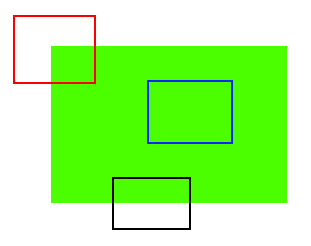
\includegraphics[scale=0.7]{Figures/feature_simple.png}
\decoRule
\caption[Ejemplo de puntos de interés]{Ejemplo sencillo de puntos característicos.}
\label{fig:feature_simple}
\end{figure}

Una vez entendido el concepto, el siguiente paso consiste en averiguar cómo encontrar estos puntos de interés en una imagen real. Por ejemplo, una manera sencilla de hacerlo es buscar las regiones en las imágenes que contienen una gran variabilidad cuando son desplazadas (una pequeña distancia) hacia todas las direcciones de los alrededores.

Existen multitud de implementaciones para calcular estas carácterísticas en las imágenes. Uno de los primeros intentos en encontrar estas esquinas fue hecho por Chris Harris y Mike Stephens \parencite{Reference8}. El método, llamado \textit{Harris Corner Detector} transforma la simple idea a una fórmula matemática (\ref{eqn:Harris}) que básicamente encuentra la diferencia en intensidad por un desplazamiento (u,v) en todas las direcciones.

\begin{equation}
E(u,v)\,=\,\sum_{x,y}w(x,y)\,\,[I(x\,+\, u,\, y\,+\, v)-I(x,y)]^{2}
\label{eqn:Harris}
\end{equation}

Donde \textit{w(x,y)} es una ventana rectangular o gaussiana e I(x,y) corresponde a la intensidad. Aplicando algunos cálculos matemáticos se llega a la ecuación (\ref{eqn:Harris}) básica que determina si una ventana contiene una esquina o no. OpenCV tiene la función \textbf{cv2.cornerHarris()} para este propósito.

%\[ R=det(m)-k(trace(M))^{2} \]
\begin{equation}
R=\lambda_{1}\lambda_{2}-k(\lambda_{1}+\lambda_{2})^{2}
\label{eqn:Harris2}
\end{equation}

$\lambda_{1}$ y $\lambda_{2}$ son los autovalores de la matriz M, que determinarán si una región es esquina, borde o zona plana.

\begin{itemize}
\item Cuando $|R|$ es pequeño, que sucede cuando $\lambda_{1}$ y $\lambda_{2}$ son pequeños, la región es plana.

\item Cuando $R < 0$, que sucede cuando $\lambda_{1} >> \lambda_{2}$ o viceversa, la región es un borde.

\item Cuando $R$ es grande, que sucede cuando $\lambda_{1}$ y $\lambda_{2}$ son grandes y más o menos iguales, la sección es una esquina.

\end{itemize}

Más tarde, J. Shi y C. Tomasi hicieron una pequeña modificación que obtuvo mejores resultados comparados con los obtenidos en el detector de Harris \parencite{Reference9}. El resultado del detector \textit{Shi-Tomasi Corner Detector} se puede ver en la ecuación~(\ref{eqn:Shi})

\begin{equation}
R=min(\lambda_{1},\lambda_{2})
\label{eqn:Shi}
\end{equation}

Si $R$ es mayor que un determinado umbral, o dicho de otro modo, solo cuando $\lambda_{1}$ o $\lambda_{2}$ se encuentran por encima de un valor mínimo $\lambda_{min}$, se considera que cierta región es esquina. En la Figura~\ref{fig:shi_detector} se puede observar el resultado de aplicar dicho algoritmo en una imagen. La función en OpenCV de este detector es \textbf{cv2.goodFeaturesToTrack()}.

\begin{figure}[ht]
\centering
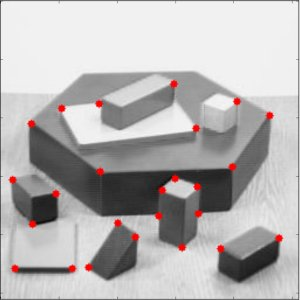
\includegraphics[scale=0.5]{Figures/shi-detector.jpg}
\decoRule
\caption[Ejemplo con \textit{Shi-Tomasi Corner Detector}]{Resultado de encontrar las mejores 25 esquinas de la imagen con \textit{Shi-Tomasi Corner Detector}.}
\label{fig:shi_detector}
\end{figure}

Existen varias implementataciones para el cálculo de carácterísticas de una imagen. A parte de las mencionadas, OpenCV proporciona entre otras \textbf{SIFT} y \textbf{SURF} que son las que hemos usado para el trabajo ya que permiten además de la detección de puntos de interés, el cálculo de descriptores. Se detallarán más adelante.

\subsection{Cálculo de descriptores}

Una vez que se conoce el punto de interés, necesitamos asignarle una huella, algo carácterístico que nos permita encontrar el mismo en otra imagen. Para ello, se procede al cálculo de descriptores (\textit{Feature Description} en inglés).

Consiste en definir la región alrededor del punto de interés para poder buscar el punto con la misma región en otra imagen. Es decir, se guarda una descripción de la región del punto dado y se busca el mismo (o el que más se parezca) a otro punto perteneciente a otra imagen.

Una vez localizado el punto se podrá llevar un seguimiento de dónde está ese punto en otra imagen. No en todos los casos se va a encontrar un descriptor perfecto para un cierto punto, por lo que al estudiar los emparejamientos se evaluará cuánto se parecen los despriptores entre sí.

\subsubsection{Descriptores SIFT}

SIFT (Scale-Invariant Feature Transform) soluciona uno de los problemas que se encontraban en los métodos anteriormente mencionados. Los métodos hasta ahora vistos para el cálculo de puntos de interés o esquinas se suponen invariantes a la rotación, es decir, incluso si la imagen es rotada es posible encontrar las mismas esquinas. Esto es así porque una esquina sigue siendo una esquina si la imagen a sido rotada. Sin embargo, no contemplan los cambios de escala, un esquina puede no ser una esquina si la imagen ha sido escalada. En la Figura~\ref{fig:sift_scale_invariant} podemos ver un ejemplo de este hecho; una esquina en una pequeña imagen con una ventana no lo es cuando la imagen se amplia y se usa la misma ventana.

\begin{figure}[ht]
\centering
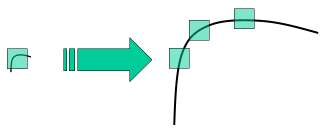
\includegraphics[scale=0.8]{Figures/sift_scale_invariant.jpg}
\decoRule
\caption[Ejemplo de sistema escalarmente variante]{Ejemplo de diferentes puntos con escala}
\label{fig:sift_scale_invariant}
\end{figure}

SIFT nace para resolver esta carencia de mano de D. Lowe \parencite{Reference10}. Un algoritmo invariante que localiza puntos de interés y calcula descriptores. Hay principalmente 4 etapas básicas en el algoritmo de SIFT:

\begin{enumerate}
\item \underline{Extrema detección en espacio-escala}

Para poder detectar características en diferentes escalas es necesario variar el tamaño de la ventana a ampliar. Para ello se utiliza un filtro de espacio-escala; un filtro LoG (Laplaciana de una Gaussiana) que con diferentes valores de $\sigma$ es capaz de detectar puntos de interés para diferentes escalas. $\sigma$ actúa como un parámetro de escala, para bajos niveles de $\sigma$ la gaussiana devuelve altos valores para las pequeñas esquinas, sin embargo, altos valores de $\sigma$ encajan bien para grandes esquinas.

Por lo tanto se busca a lo largo de la imagen y en diferentes escalas para encontrar el punto. Así pues a lo largo de la imagen y en diferentes escalas tenemos una lista de $(x,y,\sigma)$ valores, donde $(x,y)$ representa el espacio y $\sigma$ la escala.

Sin embargo, el filtro LoG es muy costoso temporalmente por lo que SIFT calcula una aproximación; la diferencia de gausianas con diferente $\sigma$ y el proceso se repetirá para diferentes octavas ($k\sigma$) como se puede apreciar en la Figura~\ref{fig:shif_dog}.

\begin{figure}[ht]
\centering
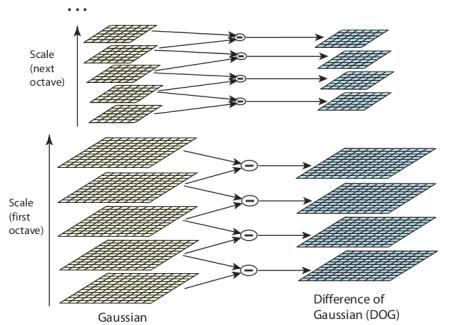
\includegraphics[scale=0.7]{Figures/sift_dog.jpg}
\decoRule
\caption[Diferencia de gaussianas en SIFT]{Proceso del cálculo de la diferencia de Gaussianas para diferentes octavas.}
\label{fig:shif_dog}
\end{figure}

Una vez obtenida la diferencia de gaussianas (DOG) se calcula el \textit{local-extrema}, por ejemplo, un píxel en una imagen es comparado con sus 8 vecinos y también con los 9 píxeles de la escala anterior y la posterior (Figura~\ref{fig:sift_local_extrema}).

\begin{figure}[ht]
\centering
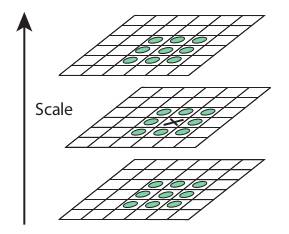
\includegraphics[scale=0.7]{Figures/sift_local_extrema.jpg}
\decoRule
\caption[Ejemplo de local-extrema en SIFT]{Ejemplo de local-extrema en SIFT.}
\label{fig:sift_local_extrema}
\end{figure}


\item \underline{Localización de puntos de interés}

Una vez que los puntos de interés se han localizado, se tienen que refinar a fin de obtener unos resultados más precisos. Por ello se elimina cualquier punto de interés de bajo contraste, definido por el umbral \textit{contrastThreshold} y los puntos caracterizados como bordes por el umbral \textit{edgeThreshold}.

\item \underline{Asignación de orientación}

En este punto cada característica obtenida de la imagen se le asigna una orientación principal para mantener el algoritmo invariante ante la rotación. Se crean puntos característicos con la misma localización y escala pero en diferentes direcciones.

\item \underline{Descriptores}

Aquí el descriptor del punto es creado con una ventana 16X16 alrededor del punto.

\item \underline{Emparejamiento de puntos}

Los puntos de interés son emparejados en base a los vecinos. Se van seleccionando emparejamientos y cuando se encuentra un emparejamiento con menor distancia se selecciona. Los emparejamientos con una distancia mayor de 0.8 se eliminan.

\end{enumerate}

La implementación de SIFT en OpenCV es sencilla, partiendo de dos imágenes en escala de grises tenemos:

\begin{lstlisting}[style=CStyle]
	SiftDescriptorExtractor extractor;
 	SiftFeatureDetector detector;
 	std::vector<KeyPoint> keypoints_1, keypoints_2;

	// Keypoints detection
 	detector.detect( img_1, keypoints_1 );
 	detector.detect( img_2, keypoints_2 );
  	
 	// Descriptors calculation
 	extractor.compute(img_1, keypoints_1, descriptors_1);
 	extractor.compute(img_2, keypoints_2, >descriptors_2);
\end{lstlisting}

\subsubsection{Descriptores SURF}

SURF (Speeded Up Robust Features) podría ser la evolución y versión rápida de SIFT. Desarrollada por Bay, H., Tuytelaars, T. y Van Gool, L. \parencite{Reference12} se introduce un nuevo algoritmo para la detección y cálculo de descriptores.

En vez de utilizar Laplaciana de la gaussiana (LoG) para encontrar el espacio de escala como SIFT, SURF va un poco más lejos y aproxima LoG con filtros de cuadros (\textit{Box Filter}). En la Figura~\ref{fig:surf1} se puede ver un ejemplo de tal aproximación.

\begin{figure}[ht]
\centering
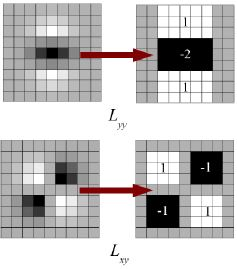
\includegraphics[scale=0.6]{Figures/surf-1.jpg}
\decoRule
\caption[Ejemplo de \textit{Box filter} en SURF]{Proceso con filtros de cuadros, \textit{Box filter}.}
\label{fig:surf1}
\end{figure}

La principal ventaja es que la convolución con cuadros es más fácil de cálcular con la ayuda de imágenes integrales. A parte, puede realizarse en paralelo para diferentes escalas.

Una vez calculado el escalado, se propone el cálculo de la orientación principal del punto de interés. Para obtener un punto invariante a las rotaciones, iluminación y orientación se utiliza \textit{wavelet de Haar} en la dirección $x$ e $y$ en una región circular de radio \textit{6s}\footnote{La \textit{s} hace referencia a un parámetro en el cómputo de descriptores de SURF que representa una escala que define los límites de las regiones circulares entorno al punto de interés.}. Después de haber evaluado las respuestas se busca la dirección predominante calculando la suma de todos los resultados dentro de una ventana con un ángulo de 60º. La región en la que se haya obtenido un mayor valor determinará la orientación buscada (Figura~\ref{fig:surf2}).

Para el cálculo del descriptor se construye una sección cuadrada en base a la orientación obtenida, alrededor del punto de interés y con un tamaño \textit{20s}x\textit{20s}. Esta región es dividida en sub-regiones de tamaño \textit{4s} x \textit{4s} y para cada una de ellas se calcula la respuesta de \textit{wavelet de Haar} de tamaño \textit{2s} tanto en $x$ como para $y$. Se genera el siguiente vector:

\begin{figure}[ht]
\centering
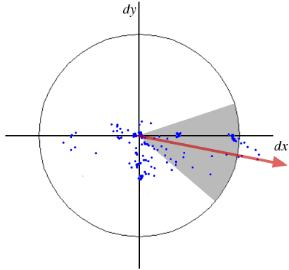
\includegraphics[scale=0.5]{Figures/surf-2.jpg}
\decoRule
\caption[Cálculo de orientación con SURF]{Cálculo de orientación con SURF.}
\label{fig:surf2}
\end{figure}

\begin{equation}
v=\left(\sum d_{x},\sum d_{y},\sum|d_{x}|,\sum|d_{y}|\right)
\end{equation}

Con el vector representado, para cada carácterística detectada el descriptor con SURF contendrá 64 dimensiones. A menor dimensión, mayor velocidad de cómputo y de emparejamiento, pero se consigue menor distinción entre características. Para esto SURF tiene una versión extendida con 128 dimensiones.

En resumen, SURF añade muchas mejoras para incrementar la velocidad en cada paso. Pruebas experimentales han demostrado que puede ser tres veces más rápido que SIFT. Aunque en robustez es comparable con SIFT, SURF se comporta bien en imágenes borrosas y con rotación pero no tanto cuando se cambian los puntos de vista o con una diferente condición de iluminación.

La implementación en código es similar a la de SIFT:

\begin{lstlisting}[style=CStyle]
	//-- Step 1: Detect the keypoints using SURF Detector
	int minHessian = 400;

	SurfFeatureDetector detector( minHessian );

	std::vector<KeyPoint> keypoints_1, keypoints_2;

	detector.detect( img_1, keypoints_1 );
	detector.detect( img_2, keypoints_2 );

	//-- Step 2: Calculate descriptors (feature vectors)
	SurfDescriptorExtractor extractor;

	Mat descriptors_1, descriptors_2;

	extractor.compute( img_1, keypoints_1, descriptors_1 );
	extractor.compute( img_2, keypoints_2, descriptors_2 );;
\end{lstlisting}



%-----------------------------------
%	SECTION Emparejamiento (\textit{matching})
%-----------------------------------
\section{Emparejamiento}

En esta sección abordaremos las distintas estrategias que se han implementado en el componente para el emparejamiento (\textit{matching}) de puntos de interés. Los emparejamientos se harán por cada fotograma que llegue de la cámara después de la extración de puntos de interés.

El componente RealRTEstimator está recibiendo continuamente imágenes del sensor, por lo que el cálculo, al igual que la extración, se hará en cada iteración. Consiguiendo así una relación entre dos fotogramas consecutivos para analizar y posteriormente cálcular el desplazamiento sucedido. Estos emparejamientos nos darán margen para desechar los peores y filtrar por mejores utilizando diferentes técnicas. Así pues, se intentará coger los mejores emparejamientos entre una imagen en $(t)$ y otra en $(t+1)$.

Se presentan dos soluciones para este problema; una primera solución que calcula el emparejamiento de puntos mediante un mecanismo de \textbf{Fuerza Bruta} y en segundo lugar el uso de la librería \textbf{FLANN}, ambas proporcionadas por OpenCV.

\subsection{Emparejamiento por Fuerza Bruta}

El mecanismo de Fuerza Bruta es simple: Se coge el descriptor de una de las carácterísticas del primer fotograma (imagen en $(t)$) y se comprueba el parecido con todos los puntos de carácterísticas del segundo fotograma (imagen en $(t+1)$). Estos emparejamientos se evalúan a través de un parámetro de distancia. De todas las características, el descriptor que más se parezca al primero o el emparejamiento que tenga la menor distancia es el devuelto.

Para el cálculo de este emparejamiento se usa OpenCV. En primer lugar se tiene que crear un objeto del tipo \textit{BruteForceMatcher} y pasarle como parámetro el tipo de medida para calcular la distancia, ya que depende del tipo de descriptor a utilizar.

Una vez creado el objeto, dos métodos importantes son \textit{.match()} y \textit{.knnMatch()}. El primero devuelve el mejor emparejamiento. El segundo devuelve los $k$ mejores emparejamientos, donde $k$ es definido por el usuario.


El siguiente ejemplo de código se puede observar cómo calcular los emparejamientos a través de OpenCV:

\begin{lstlisting}[style=CStyle]
	// matching descriptors
	BruteForceMatcher<L2<float> > matcher;
	vector<DMatch> matches;
	matcher.match(descriptors1, descriptors2, matches);
\end{lstlisting}

\textit{matches} por tanto será un array de objetos \textit{DMatch} (objeto de emparejamiento) con los siguientes atributos:

\begin{itemize}
\item \textit{DMatch.distance} - Parámetro de distancia entre descriptores. Cuanto menor distancia mejor emparejamiento.

\item \textit{DMatch.trainIdx} - Índice del descriptor de la segunda imagen con el resultado.

\item \textit{DMatch.queryIdx} - Índice del descriptor de la primera imagen a buscar.

\item \textit{DMatch.imgIdx} - Índice de la imagen resultado.
\end{itemize}

En Figura~\ref{fig:SiftDetector} podemos ver un ejemplo real de una prueba casera utilizando el algoritmo de Fuerza Bruta. Como se puede apreciar, el tener que emparejar todos los puntos de una imagen al más parececido de la otra proporciona, incluso en una imagen muy parecida, errores que se van a tener que filtrar.

\begin{figure}[th]
\centering
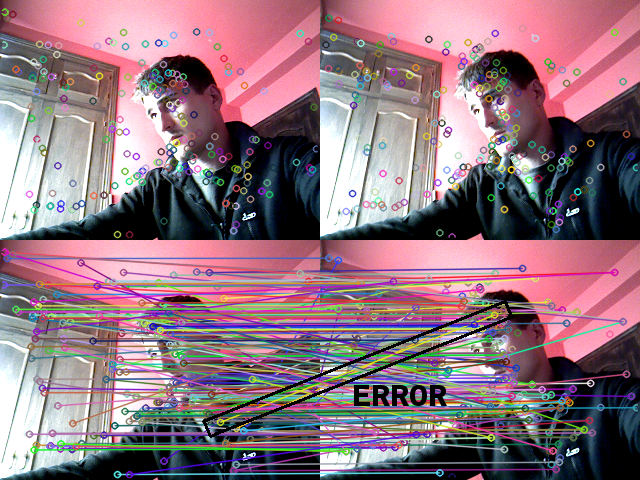
\includegraphics[scale=0.8]{Figures/sift-detector.png}
\decoRule
\caption[Captura real con SIFT]{Detección y emparejamiento de puntos de interés con OpenCV usando SIFT para el cálculo de puntos de interés y descriptores y Fuerza Bruta para el cálculo de los emparejamientos.}
\label{fig:SiftDetector}
\end{figure}



Por último, para la visualización OpenCV dispone del método \textit{.drawMatches()} que a partir de las dos imágenes y los emparejamientos obtenidos ayuda a dibujar los mismos para su visualización. Coloca las dos imágenes a tratar en horizontal y dibuja las líneas con los emparejamientos de una imágen a otra. En el caso de usar y querer visualizar los $k$ mejores emparejamientos existe también el método \textit{.drawMatchesKnn}.


\subsection{Emparejamiento por FLANN}

FLANN (\textit{Fast Library for Approximate Nearest Neighbors}) es una librería que contiene una colección de algoritmos optimizados para encontrar emparejamientos. Esta librería de OpenCV, es una implementación del trabajo de Marius Muja y David G. Lowe \parencite{Reference11}. Está pensada para trabajar con grandes conjuntos de datos y cuando los descriptores son representados por vectores de grandes dimensiones. Por lo que en estos entornos trabajará más rápido que el algoritmo de Fuerza Bruta.

FLANN provee de un sistema para elegir automáticamente el mejor algoritmo basado en la colección de datos. Dispone también de unos parámetros de entrada que permiten al usuario especificar la importancia de minimizar la memoria o el tiempo de compilación en lugar del tiempo de búsqueda.

La implementación en código con OpenCV es sencilla y muy parecida a la anterior:

\begin{lstlisting}[style=CStyle]
  //Matching descriptor vectors using FLANN matcher
  FlannBasedMatcher matcher;
  std::vector< DMatch > matches;
  matcher.match(descriptors_1, descriptors_2, matches);
\end{lstlisting}
\subsection{Resolución de errores de emparejamiento}

Sobre el filtrado de errores se han usado dos estrategias. Se han cogido de todos los emparejamientos un porcentaje relativamente pequeño donde se encuentran los emparejamientos más acertados, tomando como medida de calidad la distancia ofrecida por los diferentes algoritmos y se ha incluido un filtro de sobresaliencia para el algoritmo de Fuerza Bruta.



\begin{itemize}
\item \underline{Mejores emparejamientos}. De $k$ emparejamientos obtenidos se ha implementado una función que ordena de menor a mayor la distancia de los emparejamientos obtenidos. Después y a través de la interfaz gráfica se podrá elegir el porcentaje de emparejamientos a emplear en la fase, que por defecto es un 20\%, es decir, $(k*0.2)$ puntos emparejados finales. Cuanto menor porcentaje mayor fiabilidad, pero menores resultados a pasar en la siguiente fase.

En la Figura~\ref{fig:bestPointsSift} se puede ver el resultado de aplicar este método tras un desplazamiento horizontal. Se comprueba que el número de fallos se reduce considerablemente.

\begin{figure}[th]
\centering
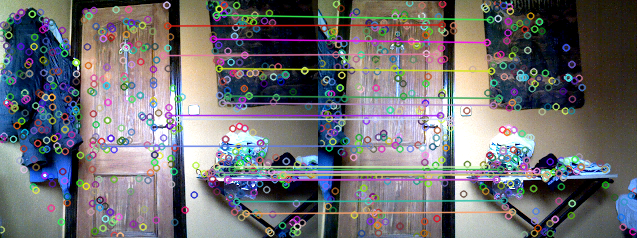
\includegraphics[scale=0.6]{Figures/best_points_sift.png}
\decoRule
\caption[Captura de los mejores puntos con SIFT]{Emparejamiento de los mejores X puntos ordenados por distancia.}
\label{fig:bestPointsSift}
\end{figure}

\item \underline{Filtro de sobresaliencia}. Este filtro surge de la necesidad de corregir un error común que se encontraba en los mejores emparejamientos por distancia. Existen ciertas situaciones en las que hay características de una imagen muy similares a otras de otra imagen y que corresponden a errores en el emparejamiento.

En la Figura~\ref{fig:similarCorrelation} se captura un ejemplo con dos de los mejores puntos medidos por distancia y se verifica que los dos mejores puntos se corresponden con el mismo punto en la imagen a buscar. Este error corresponde a una situación poco casual y es origen de muchos errores en la estimación.

\begin{figure}[th]
\centering
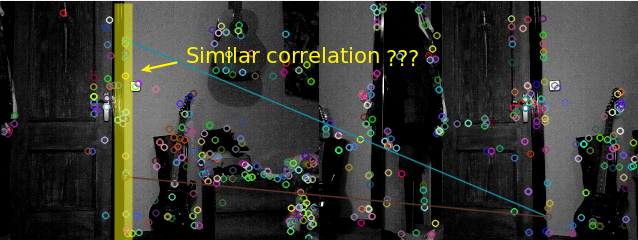
\includegraphics[scale=0.6]{Figures/similar-correlation.png}
\decoRule
\caption[Captura con error de los dos mejores puntos en SIFT]{Detección y emparejamiento de los mejores dos puntos.}
\label{fig:similarCorrelation}
\end{figure}

Se puede entender en la Figura~\ref{fig:similarCorrelation} que el punto con el resultado final del emparejamiento (imagen derecha) tiene a nivel de descriptores una mayor similitud que los demás, de ahí ese resultado. Pero los dos mejores puntos tienen una correlación muy similar, al igual que tendrán los demás puntos a lo largo del marco de la puerta subrayado en amarillo.

Para ello, se ha empleado el método \textit{.knnMatch()} en el algoritmo de Fuerza Bruta que coge los $k$ mejores puntos. En este caso, se cogen los 2 mejores emparejamientos de todos los puntos y si la diferencia entre estos dos mejores emparejamientos es muy paqueña $(< 100)$ se desecha. Así pues, este filtro garantiza que el emparejamiento obtenido a través de los dos puntos es muy fuerte y no hay otro descriptor en la otra imagen con características similares.

El código para esta implementación es sencillo:

\begin{lstlisting}[style=CStyle]
	// Filtro de sobresaliencia
	vector<vector<DMatch> > matches_vector;
	matcher.knnMatch(descriptors1, descriptors2, matches_vector, 2);
	for (int i=0; i<matches_vector.size(); i++) {
		outNumber = matches_vector[i][1].distance - matches_vector[i][0].distance;
		if (outNumber >= OUTSTANDING_DISTANCE) {
			// Guardamos el emparejamiento
		}
	}
\end{lstlisting}

Donde \textit{OUTSTANDING\_DISTANCE} es el umbral mínimo de diferencia de distancias permitido, que por defecto se ha definido en 100.

Como diferencia, en esta ocasión como resultado del método \textit{.knnMatch()} se obtiene un vector de vectores. Cada vector corresponde a un posible emparejamiento y por cada uno, otro vector con los $k$ mejores emparejamientos.

\end{itemize}

%-----------------------------------
%	SUBSECTION Obtención de puntos 3D
%-----------------------------------
\section{Obtención de puntos 3D}

Una vez obtenidos los puntos de interés y los mejores emparejamientos, se necesita llevar a 3D los puntos calculados para el instante $(t)$\footnote{Como explicaremos más adelante, no se necesitarán calcular los puntos 3D para el instante $(t-1)$ ya que los puntos en ese instante ya se habrán calculado.}, para analizar en la siguiente fase el desplazamiento en tres dimensiones.

Esos puntos de interés en dos dimensiones, o mejor llamados, píxeles, se obtienen a partir de la imagen RGB que proviene del sensor. Sin embargo, para este cálculo de puntos 3D se necesitará además la imagen DEPTH correspondiente. O lo que es lo mismo, el mismo píxel o punto de la imagen a color debe relacionarse con su homólogo en la imagen de profundidad. Se puede deducir que ambas imágenes deberán estar perfectamente sincronizadas para asegurar que ambas se corresponden con el mismo instante de tiempo. En la Figura~\ref{fig:diagramPoints3d} tenemos el diagrama de transformación de los puntos.

\begin{figure}[th]
\centering
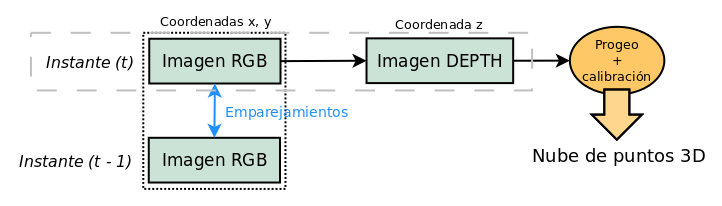
\includegraphics[scale=0.4]{Figures/diagram-points-3d.png}
\decoRule
\caption[Diagrama con la obtención de puntos 3D]{Diagrama de transformación a puntos 3D.}
\label{fig:diagramPoints3d}
\end{figure}

Para conseguir la información 3D se ha utilizado la librería de Progeo, disponible en JdeRobot, y su modelo de proyección \textit{PinHole}. Una vez obtenidos los puntos 2D más su información de distancia, se busca la recta de retroproyección correspondiente a cada uno de los píxeles de la imagen que se quieran transformar. Después se calcula el punto 3D, que será el que se encuentre a una distancia $d$ de la recta de retroproyección (ej: punto $P$ en la Figura~\ref{fig:camLine}).

\begin{figure}[th]
\centering
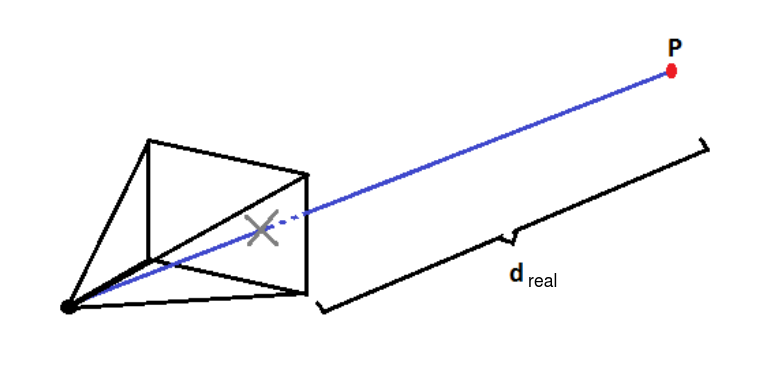
\includegraphics[scale=0.35]{Figures/cam-line.png}
\decoRule
\caption[Cálculo de punto 3D con la información de distancia $d$]{Cálculo de punto 3D con la información de distancia $d$.}
\label{fig:camLine}
\end{figure}

La transformación de un píxel a su homólogo en 3D es compleja. El proceso de recostrucción está basado en un modelo proyectivo desde el centro óptico. La distancia que devuelve el sensor, sin embargo, es la distancia perpendicular al plano imagen, y no la distancia real, tal y como se puede apreciar en la Figura~\ref{fig:distPoint}. Para ello, si se quiere calcular la posición 3D asociada a un píxel cuya recta de retroproyección es la que une el foco de la cámara y un punto BP (Figura~\ref{fig:calculate3d}) el punto que se quiere calcular no será el punto $P$, punto a una distancia $d$ del foco de la cámara y que nos da el sensor, sino el punto $Pr$ que corresponde al punto 3D real.

\begin{figure}[th]
\centering
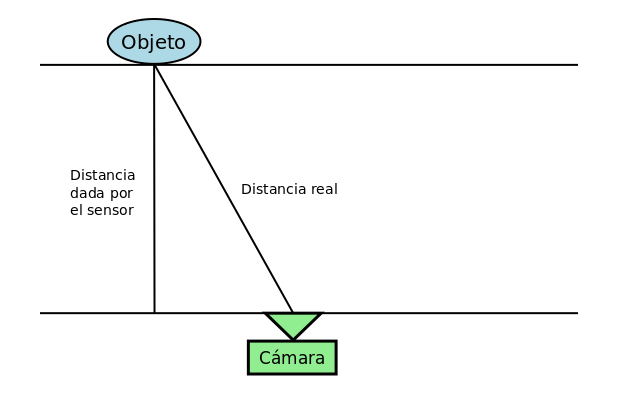
\includegraphics[scale=0.4]{Figures/dist-point.png}
\decoRule
\caption[Distancia real y la dada por el sensor]{Distancia real y la dada por el sensor.}
\label{fig:distPoint}
\end{figure}

Para calcular el punto $Pr$, se tiene que encontrar la intersección entre la recta de retroproyección y el plano $D$. Definimos el plano $D$ como el plano con vector normal $\vec{k}$ que pasa por el punto $Q$. El vector $\vec{k}$ se obtiene como vector unitario que une el centro óptico de la cámara con el foco de atención, $foa$ (\textit{focus of attention}). Este vector es un vector perpendicular al plano imagen. El $foa$ es un parámetro conocido que obtenemos en el proceso de calibración de la cámara junto con la orientación y el \textit{roll}\footnote{Movimento del sensor sobre el eje central del sensor, paralelo al $foa$ o foco de atención.} (parámetros extrínsecos). El proceso matemático es el siguiente:

\begin{figure}[th]
\centering
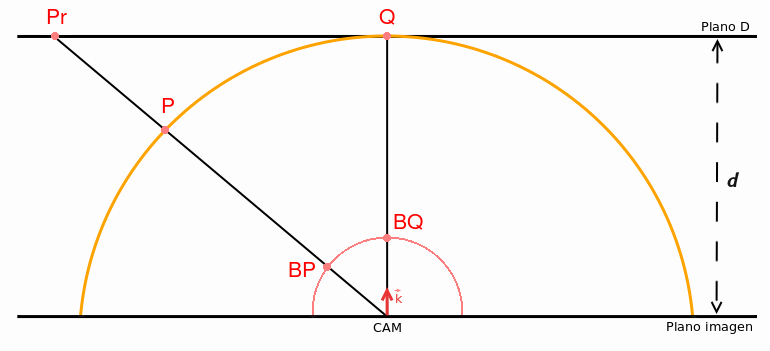
\includegraphics[scale=0.5]{Figures/calculate-3d.png}
\decoRule
\caption[Ejemplo de corrección de distancia]{Ejemplo de corrección de distancia.}
\label{fig:calculate3d}
\end{figure}

Se calcula el vector unitario $\vec{k}$ entre \textit{CAM} y $foa$:

\begin{equation}
\vec{k}=\frac{\overrightarrow{CAMFOA}}{|CAMFOA|}
\end{equation}

Una vez obtenido el vector $\vec{k}$ se obtiene el punto $Q$ que se encuentra a una distancia $d$ del sensor, con las ecuaciones paramétricas de la recta:

\begin{equation}
Q_{x}=CAM_{x}+d\cdot k_{x}
\end{equation}
\[ Q_{y}=CAM_{y}+d\cdot k_{y} \]
\[ Q_{z}=CAM_{z}+d\cdot k_{z} \]

Con esto se tendría el plano que contiene el punto $Pr$ que es el que se quiere calcular. Es decir, el punto sobre la recta que pasa por $BP$ a una distancia $D$ (distancia corregida) del punto \textit{CAM}.

Realizando los mismos cálculos, definimos el vector director de la recta \textit{CAMBP}; $\vec{v}$:

\begin{equation}
\vec{v}=\frac{\overrightarrow{CAMBP}}{|CAMBP|}
\end{equation}

Utilizando la ecuación paramétrica de la recta:

\begin{equation}
Pr_{x}=CAM_{x}+D\cdot v_{x}
\label{eqn:param}
\end{equation}
\[ Pr_{y}=CAM_{y}+D\cdot v_{y} \]
\[ Pr_{z}=CAM_{z}+D\cdot v_{z} \]


Como el punto $Pr$ se encuentra en el plano $D$, se tendrá que calcular la intersección de la recta recién calculada y el plano $D$. Para calcular el plano $D$ se aplica la ecuación del plano con los datos obtenidos; $Q$, $Pr$ y el vector normal al plano $\vec{k}$:

\begin{equation}
k_{x}(CAM_{x}+t\cdot v_{x}-Q_{x})+k_{y}(CAM_{y}+t\cdot v_{y}-Q_{y})+k_{z}(CAM_{z}+t\cdot v_{z}-Q_{z})=0
\end{equation}

Despejando $t$:

\begin{equation}
t=\frac{-k_{x}\cdot CAM_{x}+k_{x}\cdot Q_{x}-k_{y}\cdot CAM_{y}+k_{y}\cdot Q_{y}-k_{z}\cdot CAM_{z}+k_{z}\cdot Q_{z}}{k_{x}\cdot v_{x}+k_{y}\cdot v_{y}+k_{z}\cdot v_{z}}
\end{equation}

Por último, aplicando el resultado de $t$ sobre la ecuación~\ref{eqn:param} se obtiene el punto real buscado $Pr$.

%-----------------------------------
%	SUBSECTION Cálculo de movimiento
%-----------------------------------
\section{Cálculo de movimiento tridimensional}

Una vez calculados los puntos 3D, el siguiente bloque del componente realizado, RealRTEstimator, es la estimación de movimiento. En este caso hay que calcular continuamente el movimiento relativo entre los instantes $(n-1)$ y $(n)$. Esto permite ir siguiendo la trayectoria y la orientación seguida por el sensor a lo largo del tiempo.

\subsection{Matriz RT}

La trayectoria seguida se definirá por una \textbf{matriz RT} (Rotación + Translación) 4x4 de la manera que muestra la Figura~\ref{fig:matrixRT}.

\begin{figure}[th]
\centering
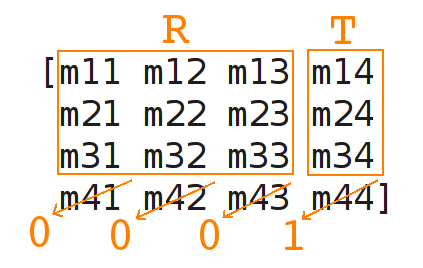
\includegraphics[scale=0.5]{Figures/matrixRT.png}
\decoRule
\caption[Matriz RT]{Matriz RT. Donde $R$ corresponde a la rotación y $T$ a la traslación.}
\label{fig:matrixRT}
\end{figure}

Donde cualquier rotación puede ser expresada como combinación ordenada de tres rotaciones por cada eje:

\begin{equation}
R_{x}(\theta)=\left[\begin{array}{ccc}
1 & 0 & 0\\
0 & cos\theta & -sen\theta\\
0 & sen\theta & cos\theta
\end{array}\right]
\end{equation}
\begin{equation}
R_{y}(\theta)=\left[\begin{array}{ccc}
cos\theta & 0 & sen\theta\\
0 & 1 & 0\\
-sen\theta & 0 & cos\theta
\end{array}\right]
\end{equation}
\begin{equation}
R_{z}(\theta)=\left[\begin{array}{ccc}
cos\theta & -sen\theta & 0\\
sen\theta & cos\theta & 0\\
0 & 0 & 1
\end{array}\right]
\end{equation}

Y tres desplazamientos:

\begin{equation}
\left[\begin{array}{c}
x'\\
y'\\
z'
\end{array}\right]=R\cdot\left[\begin{array}{c}
x\\
y\\
z
\end{array}\right]\longrightarrow\, x'=x+t_{x};\,\,\, y'=y+t_{y};\,\,\, z'=z+t_{z}
\end{equation}

Se puede deducir, por tanto, que la matriz define en total seis grados de libertad para caracterizar completamente el movimiento tridimensional.

\subsection{Cálculo RT mediante SVD}

Al calcular los puntos 3D a través de \textit{progeo} desde el sensor se tienen siempre los puntos en coordenadas \textbf{relativas}, por lo que al mover la cámara si calculamos de nuevo otros puntos estos se encontrarán en el mismo sistema de referencia. Por lo tanto, a parte de encontrar los puntos en 3D en relativas, habrá que hacer los cálculos para encontrar esos puntos en coordenadas \textbf{absolutas}.

Como sistema de referencia absoluto se toma el de la primera posición de la cámara. Así las coordenadas absolutas iniciales vienen dadas por la matriz unidad. A partir de ahí se empieza a calcular con respecto a ese sistema de referencia absoluto de los nuevos puntos en cada instante y de la cámara.

Los mismos puntos, se encontrarán en la misma posición en coordenadas absolutas en diferentes instantes de tiempo. Como se puede apreciar en la Figura~\ref{fig:movementRt} el desplazamiento del sensor en coordenadas absolutas muestra:

\begin{itemize}
\item Puntos absolutos correspondientes únicamente al instante $(n-1)$.
\item Puntos absolutos correspondientes únicamente al instante $(n)$.
\item Cámaras en absolutas correspondientes tanto al intante $(n-1)$ como $(n)$.
\end{itemize}

\begin{figure}[th]
\centering
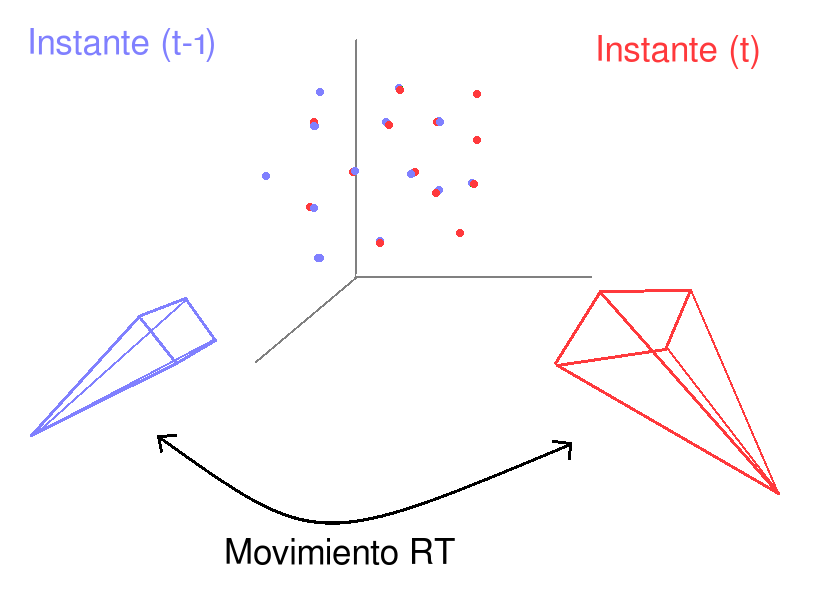
\includegraphics[scale=0.4]{Figures/movement-rt.png}
\decoRule
\caption[Cálculo visual de movimiento en coordenadas absolutas]{Cálculo visual de movimiento en coordenadas absolutas.}
\label{fig:movementRt}
\end{figure}

Esos puntos comunes son los utilizados para el cálculo de movimiento de la cámara y son los provenientes del emparejamiento entre píxeles de las imágenes.

Como entrada en este bloque de cálculo RT tendremos:

\begin{enumerate}
\item \underline{Los puntos relativos} provenientes de la cámara en el instante $(t)$.
\item \underline{Los puntos absolutos} correspondientes al instante $(t-1)$.
\end{enumerate}

La nube de puntos guardada será almacenada en un vector del siguiente tipo:

\begin{lstlisting}[style=CStyle]
    struct myPoint {
      int x;
      int y;
      jderobot::RGBPoint rgbPoint;
    };
    std::vector<myPoint> myPrevPoints;
\end{lstlisting}

donde se guardarán los píxeles y su correspondiente punto 3D en coordenadas absolutas, calculado de la iteración anterior. Con esto conseguimos la Matriz RT con un desplazamiento absoluto.

Para los cálculos de la matriz RT se ha usado la librería \textit{Eigen} con la descomposición en valores singulares (\textbf{SVD}), ya que permite resolver sistemas sobredimensionados. En concreto se ha usado la clase \textit{JacobiSVD} para la descomposición de una matriz rectangular.

Partiendo de la nube de puntos en coordenadas absolutas (mundo) del instante $(n-1)$ y la nube de puntos en coordenadas relativas (cam) en el instante $(n)$; se calcula la matriz RT de la cámara con respecto al mundo que mejor hace encajar la nube relativa en el instante $(n)$ con respecto a la absoluta en el instante $(n-1)$, tal y como expresa la siguiente ecuación:

%Para expresar un punto $P$ que viene dado en el sistema de referencia de la cámara (relativas) a sus coordenadas absolutas solo hay que multiplicar por la RT de la cámara en el mundo absoluto, tal y como expresa la siguiente ecuación:

\begin{equation}
RT_{cam}^{mundo}\cdot P_{pto(n-1)}^{mundo}=P_{pto(n)}^{cam}
\end{equation}

Una vez calculada la matriz RT de la cámara con respecto al mundo, para expresar un punto $P$ que viene dado en el sistema de referencia de la cámara (relativas) a sus coordenadas absolutas solo hay que multiplicar por la matriz obtenida, que contiene la RT de la cámara en el mundo absoluto, tal y como expresa la siguiente ecuación:

\begin{equation}
\left(RT_{cam}^{mundo}\right)^{-1}\cdot P_{pto(n)}^{cam}=P_{pto(n)}^{mundo}
\end{equation}

En este caso para calcular la nube de puntos del instante actual y con coordenadas absolutas solo se tiene que multiplicar por la inversa de la matriz calculada.

Una vez llegados a este punto se guarda el resultado correspondiente para los cálculos de la siguiente iteración:

\begin{equation}
P_{pto(n)}^{mundo}\longrightarrow P_{pto(n-1)}^{mundo}
\end{equation}

donde la nube de puntos absolutas, recién calculada, en $(n)$, pasa a ser la nube de puntos absolutas en $(n-1)$.
\subsection{Optimización mediante RANSAC}

El cálculo de movimiento ha sido uno de los puntos en los que se ha encontrado más problema ya que el error es acumulativo y una iteración con un error demasiado grande produce que en los siguientes instantes el cálculo de la posición absoluta de la cámara sea erróneo y arrastre indefinidamente ese error. Por ello, hay que asegurarse de que todos los datos que vienen de los anteriores bloques, vengan con el menor error posible.

Para corregir el error en esta fase se ha optado por añadir dos filtros:

\begin{itemize}
\item Deshacer el cálculo con demasiado error espacial y de reproyección.
\item Implementación de \textbf{RANSAC} para eliminar fallos espúrios.
\end{itemize}

El método de RANSAC (\textit{Random Sample and Consensus}) nos ayuda con el ruido y los datos atípicos. Clasifica los datos en dos subconjuntos: uno de ellos son los datos que satisfacen un patrón o un modelo que consideramos bueno y otro subconjunto que corresponde con los datos malos o atípicos.

Esta discriminación permitirá en gran medida conseguir una solución que se adapte al conjunto de datos que nos interesa conseguir.

Los distintos parámetros de los que consta el algoritmo que se ha implementado son:

\begin{itemize}
\item Parámetros a elección del usuario, que en código están definidos como:

\begin{enumerate}
\item \textit{RANSAC\_PERC}: Es el porcentaje de emparejamientos que se esperan que sean buenos.
\item \textit{RANSAC\_ITER}: Corresponde al número de iteraciones que ejecuta el algoritmo.
\end{enumerate}
\item Parámetros propios del algoritmo:

\begin{enumerate}
\item $N$: Número total de emparejamientos 3D.
\item \textit{good\_sub}: Subconjunto de datos buenos.
\item \textit{bad\_sub}: Subconjunto de datos malos o atípicos.
\end{enumerate}
\end{itemize}

Para lograr esto, el algoritmo de RANSAC implementado hace lo siguiente:

\begin{enumerate}
\item Del número total de emparejamientos ($N$) se selecciona un porcentaje aleatorio (\textit{RANSAC\_PERC}). Este parámetro definido por el usuario determina el porcentaje de puntos en los que se supone que siempre va a haber un subconjunto bueno de datos. Cuanto más porcentaje más puntos para poder hacer la estimación de movimiento 3D, pero más posibilidad también de tener valores erróneos. Por lo tanto,  habrá que escoger dependiendo del número medio de emparejamientos, así como su porcentaje de error para cada iteración.

\item Con los $N$ emparejamientos seleccionados, se realiza la estimación de la matriz de movimiento 3D mediante SVD.

\item A partir de la matriz RT obtenida del paso anterior se coge la nube de puntos proveniente de la cámara y le aplicamos la RT para transformarlas a coordenadas absolutas. Para cada punto 3D transformado se calcula la distancia o el error que existe entre ese punto y el mismo en el instante anterior y se van sumando. El resultado de la suma de error o distancia total se mantiene guardado.

\item Se repiten los pasos 1, 2 y 3 tantas veces como esté definido en \textit{RANSAC\_ITER}. Este parámetro cuanto mayor sea, mayor probabilidades de encontrar un subconjunto mejor, por contra, el número de iteraciones compromete el tiempo de cómputo.

Para cada iteración completa, se comprueba la distancia total obtenida en el paso 3. Si es menor se guarda, si no, se desecha.
 
\item De todas las iteraciones se selecciona la que ha tenido una menor distancia o error y se guarda la matriz RT utilizada.

\item Se emplea la matriz RT del paso 4 para calcular la nube de puntos final.

\end{enumerate}

Para el \textbf{error espacial} se ha medido la distancia entre los mismos puntos en el sistema de referencia absoluto para los instantes $(n-1)$ y $(n)$. 

Para el \textbf{error de reproyección} se mide la distancia entre píxeles de los diferentes instantes. Se calcula con \textit{Progeo} la posición del nuevo píxel en el instante anterior para poder calcular la distancia para una misma imagen.

Este algoritmo es muy robusto frente a valores espurios, ya que si se realiza el cálculo con alguno de estos valores o puntos ruidosos se desechará el resultado cogiendo como matriz RT la de otra iteración de RANSAC.

%-----------------------------------
%	SECTION Interfaz gráfica
%-----------------------------------
\section{Interfaz gráfica}

El componente desarrollado dispone de una interfaz gráfica en donde se pueden ver gráficamente los pasos realizados individualmente, así como el resultado final de toda la lógica del sistema. Ha sido desarrollada con \textit{glade} y la apariencia se puede observar en la Figura~\ref{fig:supergui}.

\begin{figure}[th]
\centering
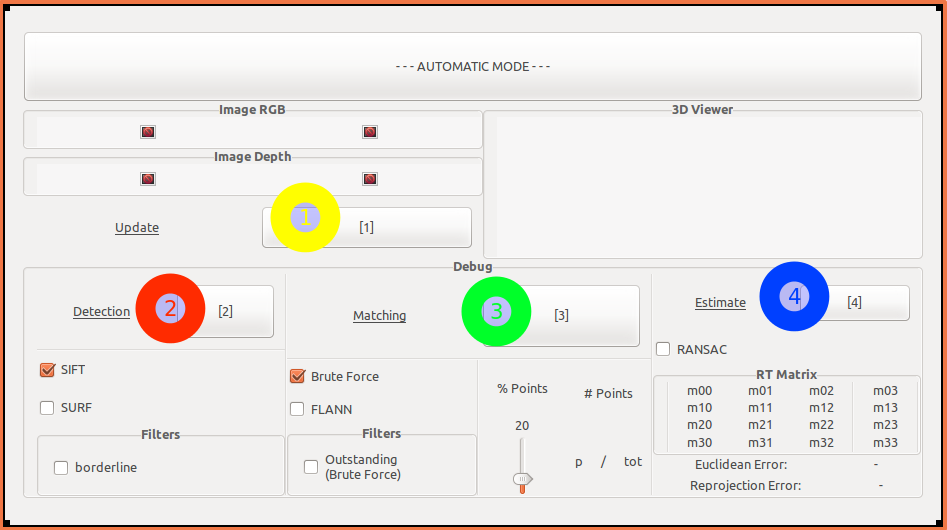
\includegraphics[scale=0.48]{Figures/super_gui.png}
\decoRule
\caption[Captura del mapa de funcionalidades de la herramienta gráfica]{Captura del mapa de funcionalidades de la herramienta gráfica.}
\label{fig:supergui}
\end{figure}

La interfaz gráfica, basada en GTK, permite la realización  del procesado paso a paso, (muy útil para depurar) o de manera automática (funcionamiento continuo). La ventana del componente teine cuatro zonas diferenciadas: 

\begin{enumerate}
\item Actualización de imagen. (Figura~\ref{fig:gui1})

\begin{figure}[th]
\centering
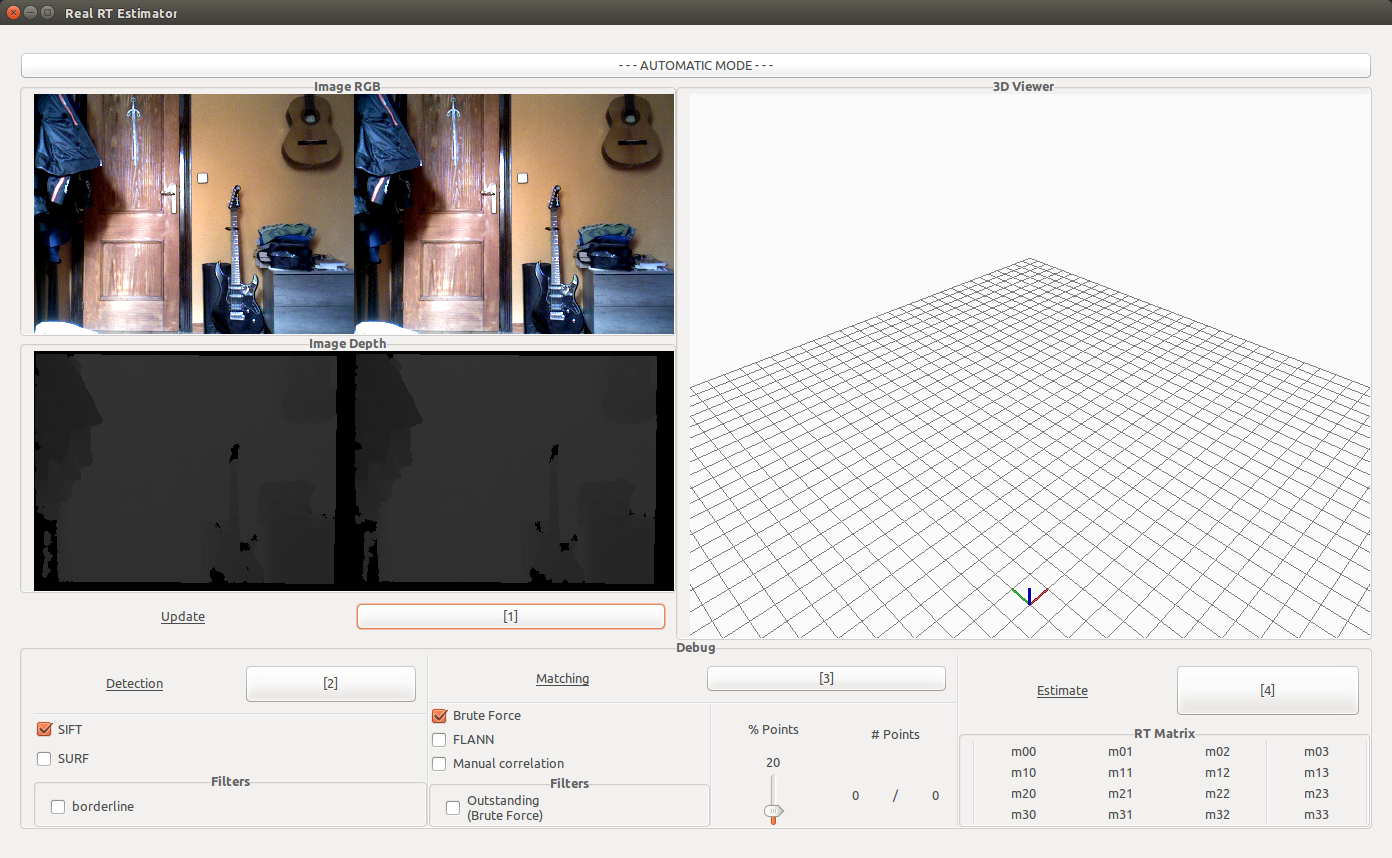
\includegraphics[scale=0.3]{Figures/gui1.png}
\decoRule
\caption[gui1]{Paso 1: Actualización de imagen.}
\label{fig:gui1}
\end{figure}

\item Detección de puntos. (Figura~\ref{fig:gui2})

\begin{figure}[th]
\centering
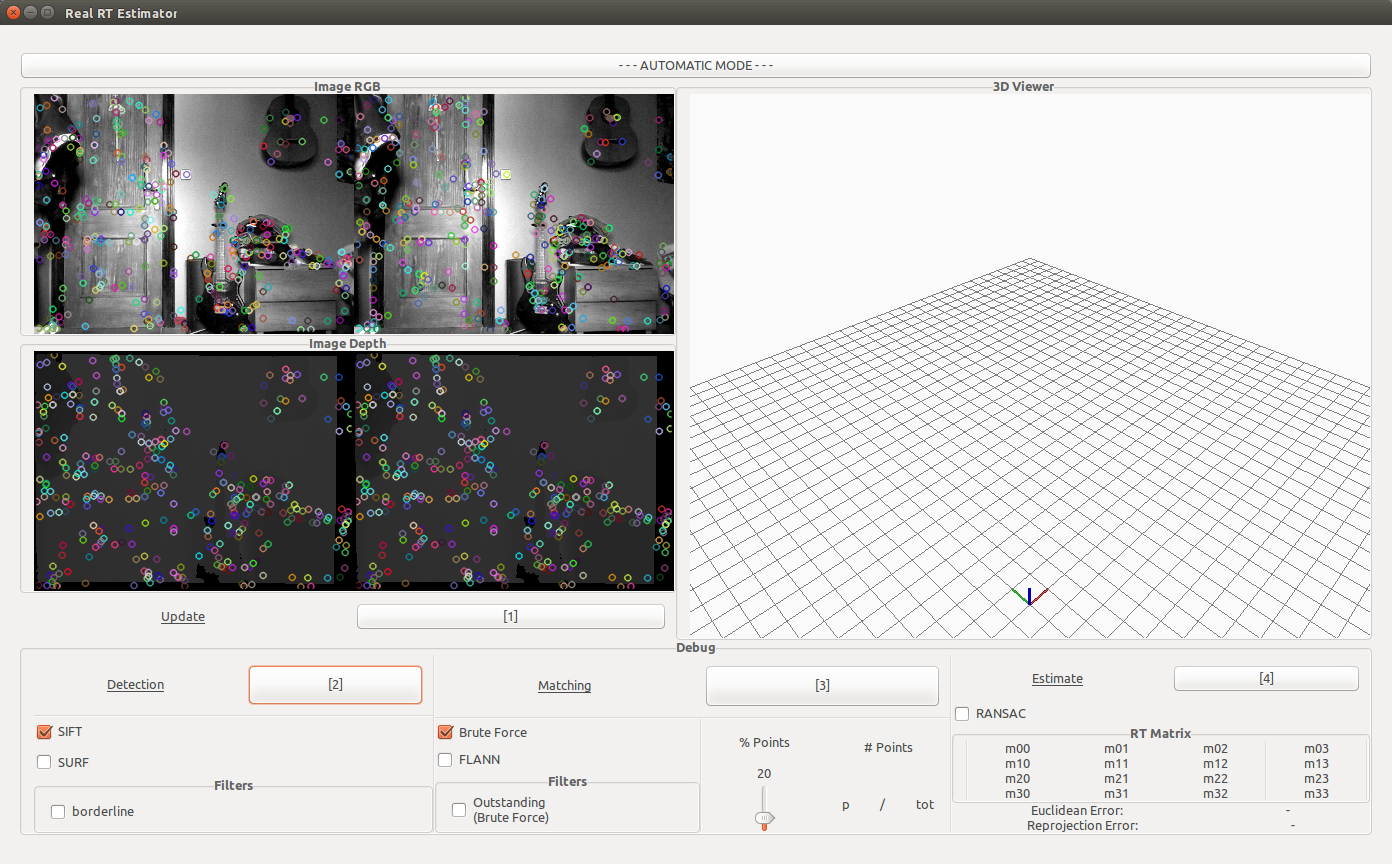
\includegraphics[scale=0.3]{Figures/gui2.png}
\decoRule
\caption[gui2]{Paso 2: Detección de puntos.}
\label{fig:gui2}
\end{figure}
 
\item Cálculo de emparejamientos. (Figura~\ref{fig:gui3})

\begin{figure}[th]
\centering
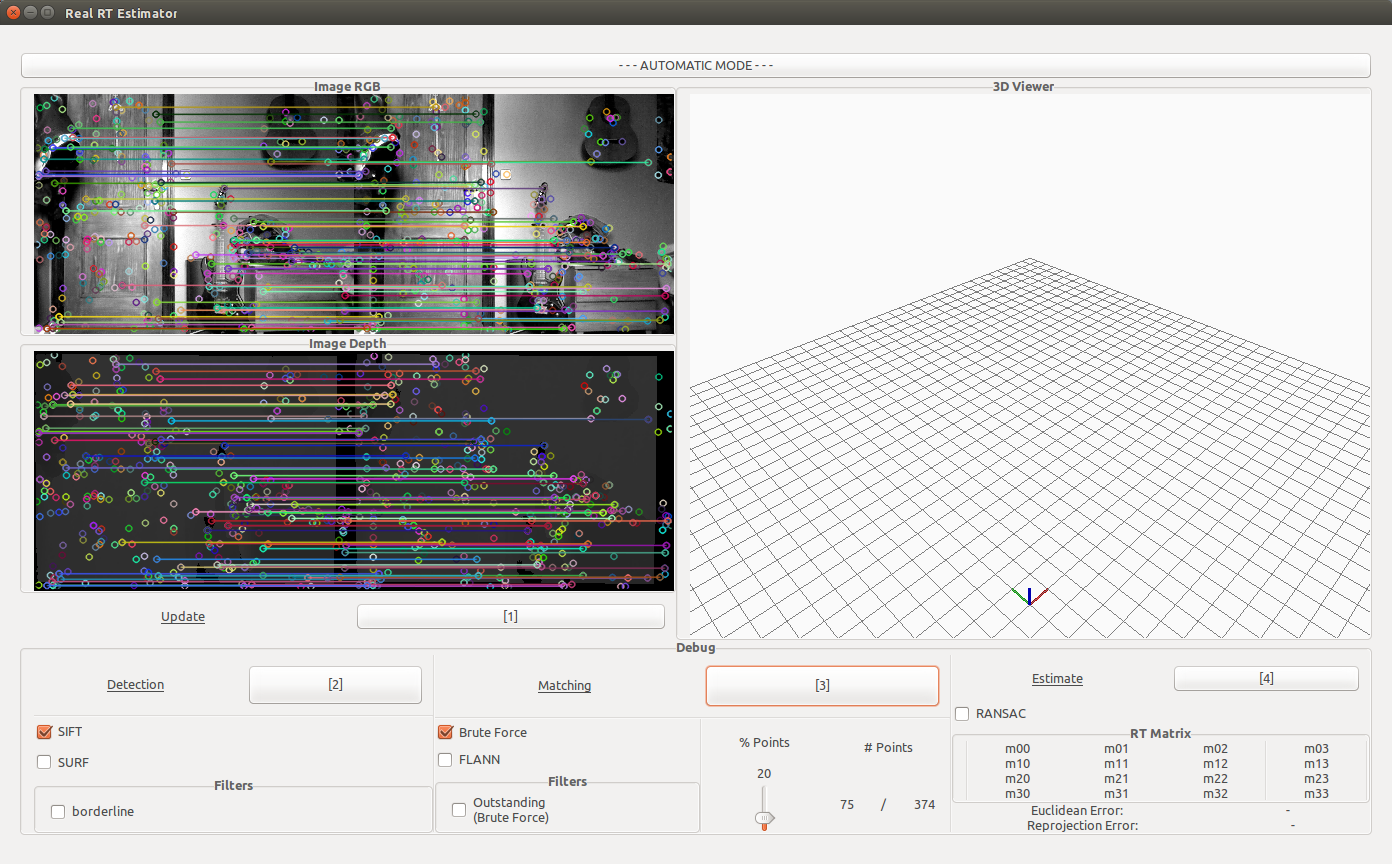
\includegraphics[scale=0.3]{Figures/gui3.png}
\decoRule
\caption[gui3]{Paso 3: Cálculo de emparejamientos.}
\label{fig:gui3}
\end{figure}

\item Estimación de la matriz. (Figura~\ref{fig:gui4})

\begin{figure}[th]
\centering
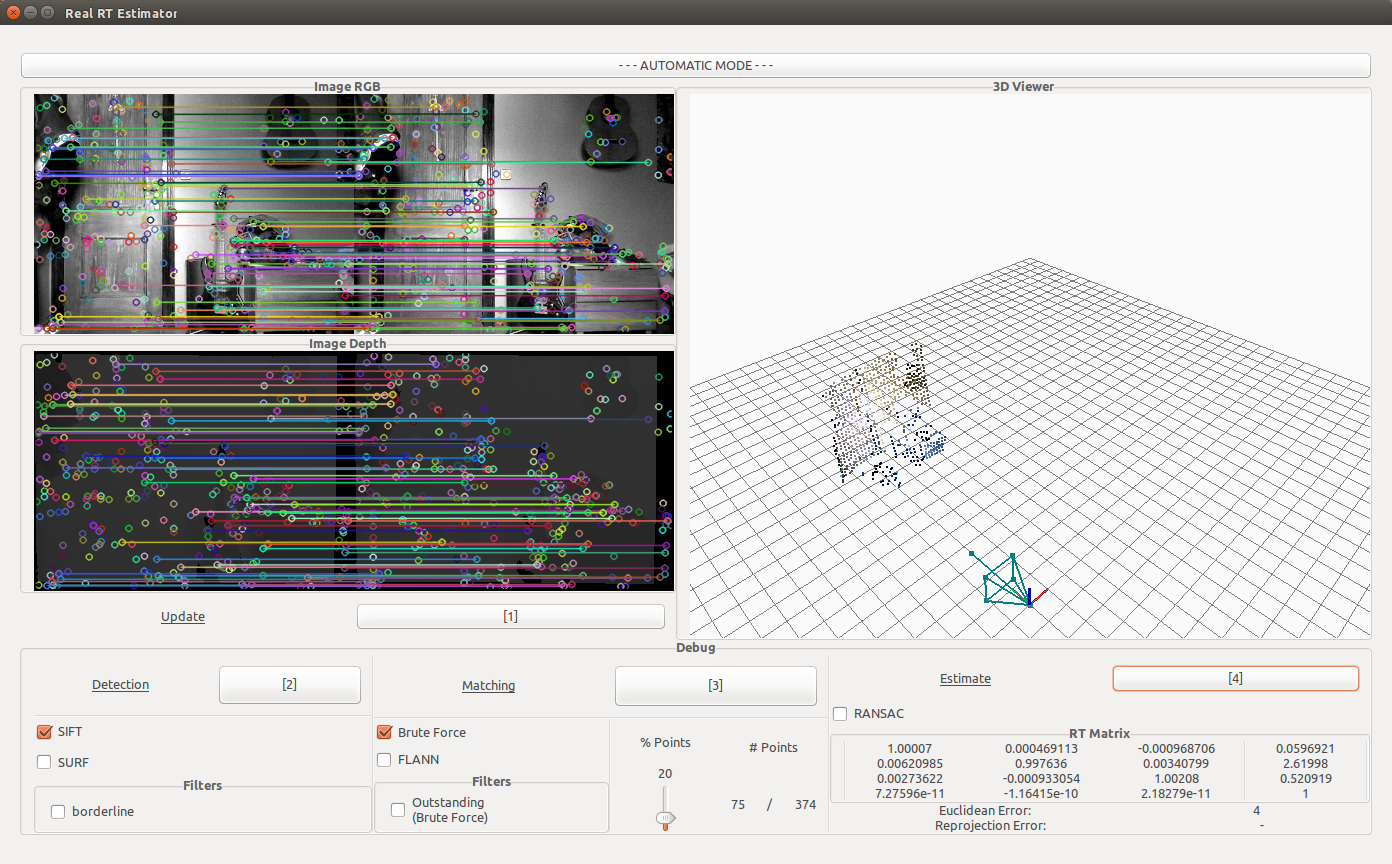
\includegraphics[scale=0.3]{Figures/gui4.png}
\decoRule
\caption[gui4]{Paso 4: Estimación de la matriz.}
\label{fig:gui4}
\end{figure}

\end{enumerate}

La herramienta permite, además, la modificación de algunos parámetros de configuración sobre la marcha, como pueden ser la elección algoritmos o filtros para el bloque de detección o el bloque de emparejamiento, así como el porcentaje de puntos emparejamientos a calcular.

Por último se ha implementado un visor 3D, donde se representa toda la información tridimensional para el sistema de referencia absoluto.

En las siguientes Figuras(\ref{fig:gui1}, \ref{fig:gui2}, \ref{fig:gui3}, \ref{fig:gui4}) se observa las capturas de cada uno de los pasos en la estimación de movimiento 3D. El botón [1] actualiza la imágen, el botón [2] detecta los puntos de interés con las opciones seleccionadas, el botón [3] los emparejamientos, un \textit{slider} para elegir el número de emparejamientos y por último el botón [4] para estimar la matriz, donde se puede observar en vivo la matriz RT estimada.

%-----------------------------------
%	SECTION Ajuste de parámetros
%-----------------------------------
%\section{Ajuste de parámetros}
%
%En el capítulo anterior hacemos referencia a algunos de los parámetros configurables que se han ido implementado a fin de poder probar el sistema con distintas configuraciones.
%
%\subsection{Parámetros Internos}
%
%Internamente existen diferentes constantes globales que permiten la configuración interna de los diferentes algorimos empleados.
%
%\subsection{Parámetros seleccionables por el usuario}
%
%A fin de poder probar el componente con diferentes algoritmos o mejorar el funcionamiento del sistema con la opción filtros, se ha implementado en la intertaz gráfica de usuarios diferentes parámetros configurables.